\documentclass{report}
\usepackage[utf8]{inputenc}
\usepackage{amsmath}
\usepackage{amssymb}
\usepackage{graphicx}

\title{Algoritmer og Datastrukturer Eksamen}
\author{Eksamensnummer: 137}
\date{\today}

\begin{document}
\maketitle

% ############################# OPGAVE 1 ####################################

\section*{Opgave 1}
\subsection*{Del 1.1}
En Fibonacci heap, $H$, er en mængde af rodfæstede træer der overholder \textit{min-heap property}'en - at nøglen i en knude er større eller lig med forældrens nøgle, hvilket resulterer i, at én af knuderne har den mindste nøgle med den mindste værdi i hele heap'en - den såkaldte  \textit{minimum node}. Vi tilgår en Fibonnaci heap med pointer'en \textit{H.min}, der pejer til denne  \textit{minimum node}. Træernes rødder har pejerene \textit{left} og \textit{right} der henholdsvis pejer til rødderne for træerne til højre og venstre for sig selv - dette skaber den såkaldte \textit{root list}. \\
Alle knuder har en pejer, \textit{p}, til sin forældre og en pejer, \textit{child}, til ét af sine børn; børnene er sammensat i en \textit{circular, doubly linked list}, hvilket herved gør det muligt for forældren at tilgå enhver af sine børn. Alle børn har pejerne \textit{left} og \textit{right}, der ved hjælp af den \textit{circular, doubly linked list} pejer til barnets højre og venstre søskene. Herudover har alle knuder attributen \textit{degree}, der beskriver antallet af børn som knuden har. \\
Herudover har alle knuder attributen \textit{mark}, der indikerer om en knude har mistet et barn siden knuden selv var lavet til et barn af en anden knude - dog bliver rodknuder ikke markeret, hvis når den mister et barn. En knude bliver \textit{unmarked} når den bliver lavet til et barn af en anden knude (hvilket kan ske når den mister sit andet barn), samt når den bliver skabt. \\
Fibonnaci heaps er en meget effektiv datastruktur, idet størstedelen af operationerne i amortiseret køretid kører i konstant tid - de eneste operationer der ikke kører i konstant tid er \texttt{EXTRACT-MIN} og \texttt{DELETE}, der har køretiderne $O(\lg n)$ og $O(\lg n)$ amortiseret køretid. Herved egner datastruktureren sig godt til algoritmer der anvender datastrukturerens operationer mange gange - og særlig godt, hvis \texttt{EXTRACT-MIN} og \texttt{DELETE} ikke anvendes særlig mange gange. Dette ses eksempelvis fra pensum i Prims algoritme og i Dijkstras algoritme. \\
Ved brugen af binære heaps har Prims algoritme en køretid på $O(E \lg V)$. Anvender algoritmen dog Fibonnaci heaps istedet, får algoritmen en køretid på $O(E + V \lg V)$, hvilket er bedre end implementationen med binære heaps, hvis tilfældet er, at antallet af knuder er meget mindre end antallet af kanter. \\
Dijkstras køretid afhænger af hvordan \textit{min-priorty} køen bliver implementeret - implementeres den ved hjælp af Fibonnaci heaps, bliver køretiden $O(V \lg V + E)$ - meget bedre end andre implementationers køretid, som for eksempel $O(V^2)$. Dette skyldes, at algoritmen generelt kalder \texttt{DECREASE-KEY} mange flere gange, end algoritmen kalder \texttt{EXTRACT-MIN}.

\newpage

\subsection*{Del 1.2}
Jeg har følgende algoritme for \texttt{INCREMENT}:
\begin{verbatim}
INCREMENT(A):
    i = 0
    while (i < A.length and A[i] == 9):
        A[i] = 0
        i += 1
    if (i < A.length):
        A[i] += 1
\end{verbatim}
Algoritmen fungerer ved at iterere igennem array $A$ indtil der findes en indgang der ikke er lig 9 - alle indgange op til dette sættes til 0, idet at lægge 1 til 9 resulterer i 0. Herefter lægges der 1 til den første værdi der ikke er lig 9, idet der herved er tale om et \textit{carry over} fra det forrige ciffer.

\newpage

\subsection*{Del 1.3}
Worst-case for algoritmen er hvis algoritmen får givet et array, hvor alle indgange er 9, altså hvor $A[i] = 9$ for $i = 0, 1, ..., 9$. Herved er while-loop'et i linje 2 nødt til at itere igennem hele array'et, hvilket giver en køretid på $O(k)$. \\
Acconting metoden til at vise den amortiserede køretid for \texttt{INCREMENT} kan vises, ved at lade de amortiserede omkostninger for at sætte et ciffer til 1, til at koste 10 credits - 1 credit bruges til at lægge 1 til cifferet, hvorimod de 9 overskydende gemmes på cifferet, som bruges til at betale for de næste 9 gange der skal lægges 1 til dette ciffer. Herved vil ethvert tal der ikke er lig 0, have nok credit til at sættes til 0 og der er derved ingen omkostninger ved at sætte et ciffer til 0, idet vi kan bruge de restende credit der ligger på cifferen. \\
Hertil kan vi bestemme den amortiserede køretid; at lægge 1 til et ciffer, udover hvis dette ciffer giver 1, bliver betalt af det credit der ligger på cifferet. Algoritmen lægger højst 1 til ét ciffer, i linje 6, hvilket betyder, at de amortiserede omkostninger maksimalt kan koste 9 (hvis cifferet går fra 0 til 1). Antallet af ciffer med credit kan ikke være negativt, hvilket betyder, at credit'et aldrig vil være negativt. Herved, ved kald til $n$ kald til \texttt{INCREMENT}, er de amortiserede omkostninger lig $O(n)$.

\newpage

% ################################### OPGAVE 2 ############################

\section*{Opgave 2}
\subsection*{Del 2.1}
Dynamisk Programming minder meget om \textit{Divide-and-Conquer}, idet begge paradigmer løser et problem, ved at dele problemet op i delproblmmer, efterfulgt af at løse disse delproblemer og tilsidst at kombinere disse delproblemer. Modsat problemer i \textit{Divide-and-Conquer}, så overlapper delproblemerne. Dette ses eksempelvis ved beregning af et Fibonacci tal:
\begin{center}
    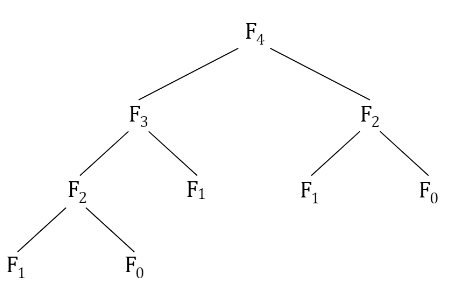
\includegraphics[height = 4 cm]{../entities/DP_fibonacci.PNG}
\end{center}
I dette eksempel er det tydeligt, at problemet består af overlappende delproblemer, idet Fibonacci-tallet $F_2$ skal udregnes 2 gange, for at udregne Fibonacci-tallet $F_4$. Ideen med Dynamisk Programmering er hertil at undgå at løse de overlappende delproblemer flere gange. \\
Ved Dynamisk Programmering er der to forskellige fremgangsmåder til, at løse et problem; \textit{top-down} og \textit{bottom-up}. \\
Ved \textit{top-down} løses problemerne rekursivt. Når et delproblem er løst, gemmes løsningen i hukommelsen og kan nemt slås op, hvis det samme delproblem er mødt igen senere. \\
Ved \textit{bottom-up} løses delproblemerne efter stigende størrelse efterfulgt af at gemme løsningen til disse delproblemer i hukommelsen. Herved, når et algoritmen støder på et nyt delproblem, er de delproblemer som den består af allerede løst. \\
Sammenlignes de to fremgangsmåder, så er det tydeligt, at de har sine fordele. \textit{top-down} har den fordel, at den kun løser den delproblemer der er nødvendige for de aktuelle problem - modsat \textit{bottom-up}, der løser alle delproblemer. På den anden side, så undgår \textit{top-down} rekursion, hvilket generelt resulterer i mindre konstantfaktorer i køretiden.

\newpage

\subsection*{Del 2.2}
Det er tydeligt, at rekursionsformlen er korrekt, idet den kører rekursivt igennem alle de mulige snit som der kan lægges på pladen og hertil finder ud af hvilke af disse snit der giver den største fortjeneste. Hertil finder rekursionsformlen altså den optimale løsning til alle de mulige delproblemer, som den finder ved at finde den optimale løsning til alle de mulige deldelproblemerne osv... Herved opnår problemet optimal delstruktur. \\
Hertil er det muligt at se, at $r_{b, h, s} = p_{b, h}$ når $b = h = 1$, idet det ikke er muligt at lægge et snit i pladen, så delpladerne har en heltalsbredde og heltalshøjde, samt $1 < b$ og $1 < h$. Det vil altså sige, at den eneste muligt i rekursionsformlen er, at returnere fortjenesten når der ikke skæres i pladen, altså, når $r_{b, h, s} = p_{b, h}$.

\newpage

\subsection*{Del 2.3}
\begin{verbatim}
CUT-PLATE(p, b, h, s):
    MANGLER
\end{verbatim}

\newpage

% ####################################### OPGAVE 3 #################################

\section*{Opgave 3}
\subsection*{Del 3.1}
Grådige Algoritmer er en type af algoritmer, der foretager sig den optimale handling i det nuværende tidspunkt, i håb om, at dette fører til det optimale løsning til hele problemet. Ligesom ved Dynamisk Programmering, så afhænger delproblemerne af andre delproblemers løsning, forskellen ligger dog i, at ved Dynamisk Programmering, foretages der et valg efter delproblemerne er løst, hvorimod en Grådige Algoritmer først foretager sig et valg og derefter løser delproblemerne. Samtidigt gælder der også, at efter hvert grådige valg, er der kun ét delproblem tilbage. Oftest er grådige algoritmer hurtigere end algoritmer fra Dynamisk Programmering, dog findes der problemer, som Dynamisk Programmering kan løse, som en Grådig Algoritme ikke kan løse. \\ 
Det kan være svært, at forudse, om et problem kan løses ved hjælp af en Grådig Algoritme. Dog, hvis et problem opnår \textit{greedy-choice property} og \textit{optimal substructure} er det muligt at løse problemet ved hjælp af en Grådig algoritme. \\
\textit{Greedy-choice property} går i sin helhed ud på, at der findes en optimal løsning til problemet, der indeholder det grådige valg. Modsat, så går \textit{optimal substructure} ud på, at hvis det grådige valg er en del af den optimale løsning til problemet, så er den optimale løsning til problemet bestående af det grådige valg og den optimale løsning til delproblemet efter det grådige valg. Alt i alt, så vil en kombination af \textit{optimal substructure} og \textit{greedy choice property} medføre, at den Grådige Algoritme finder en optimal løsning til problemet.

\newpage 

\subsection*{Del 3.2}
Af hensyn til klarheden af håndkørlsen, opstiller jeg først her de forskellige elementer:
\begin{center}
    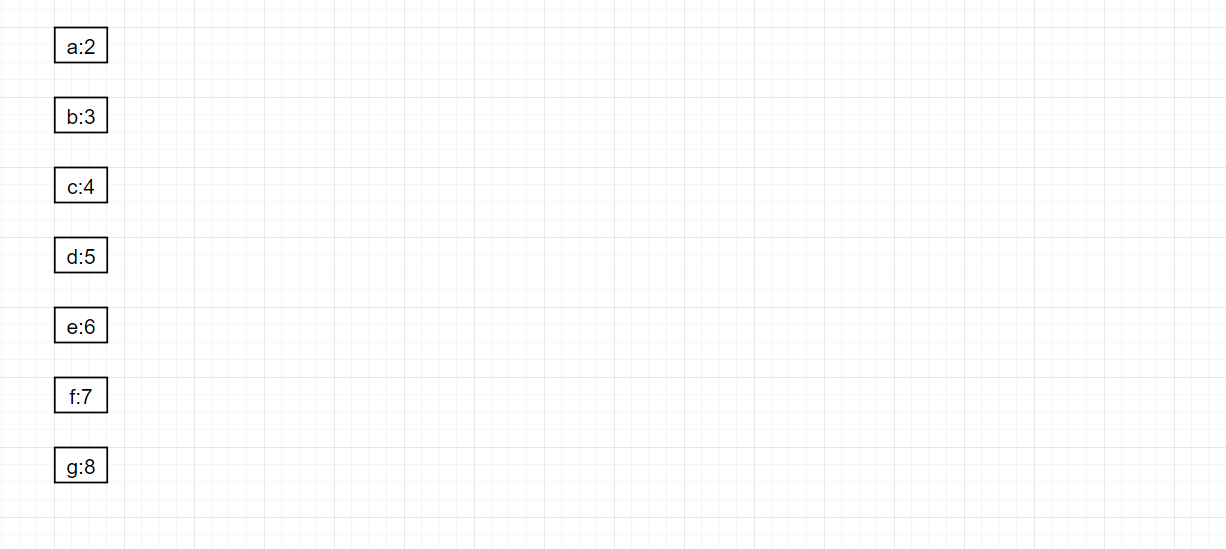
\includegraphics[height = 5 cm]{../entities/huffman1.PNG}
\end{center}
Herefter tages først de 3 knuder med lavest frekvens. Disse tre knuder bliver samlet i et træ og sumen af deres frekvenser bliver indskrevet i roden:
\begin{center}
    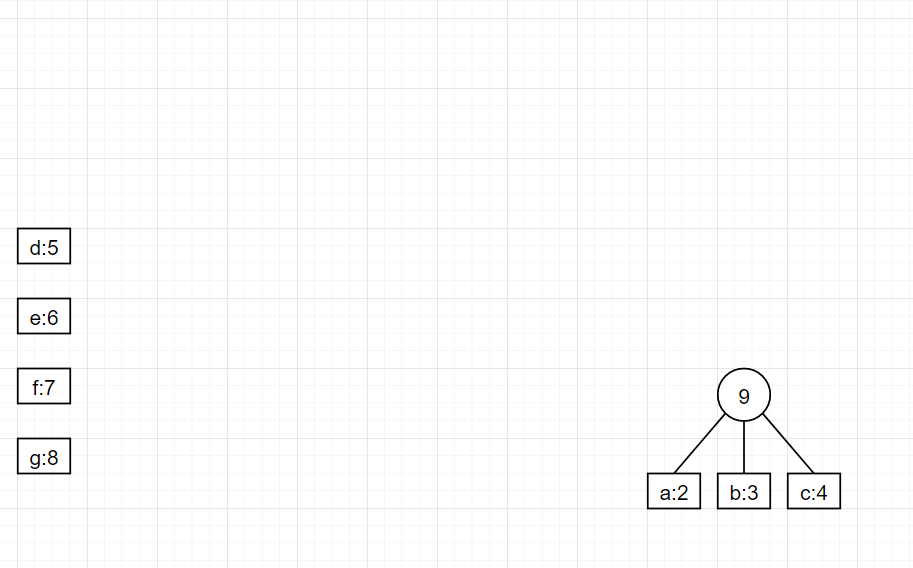
\includegraphics[height = 5 cm]{../entities/huffman2.PNG}
\end{center}
Herefter tages de 3 næste knuder med lavest frekvens. Også disse tre knuder bliver samlet i et træ og sumen af deres frekvenser bliver også indskrevet i roden:
\begin{center}
    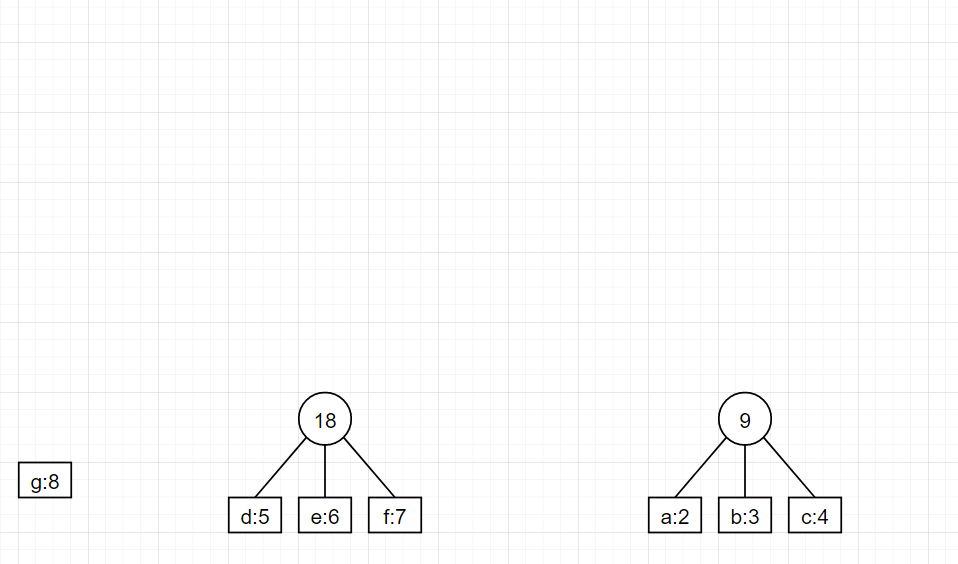
\includegraphics[height = 5 cm]{../entities/huffman3.PNG}
\end{center}
Hertil tager jeg igen de tre knuder med lavest frekvens. I dette tilfældet er det bogstavet \textit{g} og de to træer fra de forrige to iterationer. Disse samles til et nyt træ, og sumen af deres frekvens skrives i roden.
\begin{center}
    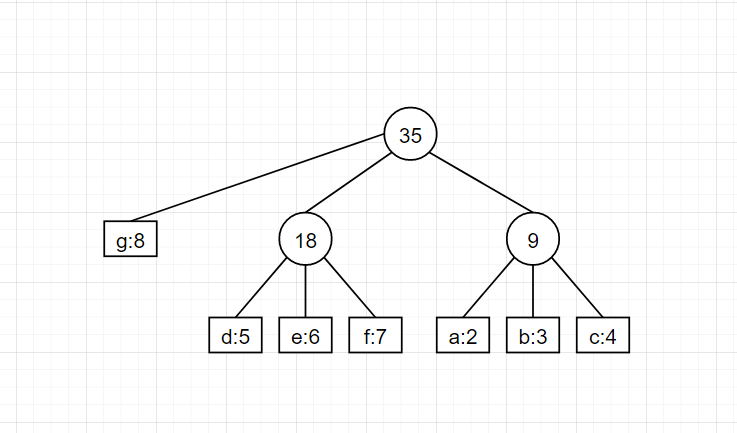
\includegraphics[height = 5 cm]{../entities/huffman4.PNG}
\end{center}
Til sidst får hver kant tilskrevet en vægt. 0 betyder "pej til barn nummer 0", 1 betyder "pej til barn nummer 1" og 2 betyder "pej til barn nummer 2".
\begin{center}
    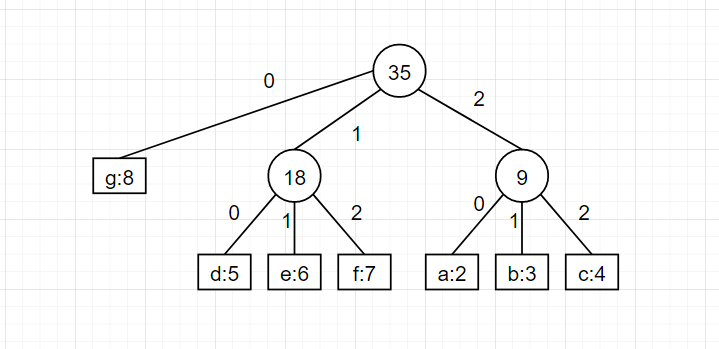
\includegraphics[height = 5 cm]{../entities/huffman5.PNG}
\end{center}
Alt i alt har de forskellige bogstaver følgende prefix-kode:
\begin{itemize}
    \item \textit{a}: 20
    \item \textit{b}: 21
    \item \textit{c}: 22
    \item \textit{d}: 10
    \item \textit{e}: 11
    \item \textit{f}: 12
    \item \textit{g}: 0
\end{itemize}

\subsection*{Del 3.3}
Vi kan implementere algoritmen, ved at skabe et \textit{min-heap}, hvor nøglerne i knuderne er frekvenserne af de forskellige bogstaver - dette har en køretid på $\Theta(n)$. Herved kan vi finde det mindste element i $O(\lg n)$. Da vi iterer over alle knuderne gøres dette $\Theta(n)$ gange. I alt har algoritmen altså en køretid på $O(n \lg n)$.

\newpage

\subsection*{Del 3.4}
Ja, $B(T) = \sum_{c \in C} c.freq \cdot d_T(c)$ udtrykker stadig længden af den komprimerede streng. Dette skyldes, at for $c \in C$ beskriver $c.freq$ antallet af gange vi går ned igennem træet til bladet hvor knuden $c$ befinder sig i, samt $d_T(c)$ beskriver hvor langt ned der er til dette bladet. Summeres dette over alle bogstaver, har vi altså hvor langt vi skal bruge for at komme til ethvert bogstav, samt hvor mange gange vi skal ned af træet, for at komme til hvert bogstav.

\newpage

\subsection*{Del 3.5}
Ved beviset skal der vises, at det grådige valg resulterer i en optimal løsning, hvor det grådige valg består af at finde de tre knuder med lavest frekvens, lave dem til søskende samt lade dem være de knuder med den største dybde. \\
Til beviset lader vi $C$ være et alfabet, hvor hvert bogstav $c \in C$ har frekvensen $c.freq$. Hertil lader vi $x$, $y$ og $z$ være de to bogstaver i $C$ med lavest frekvens. Hertil lader vi $a$, $b$ og $c$ være de bogstaver og søskende med maksimum dybde i et træ $T$ der repræsenterer et optimalt \textit{prefix code}. \\
Vi kan lave $T$ om til $T'$, ved at bytte om på knuderne $a$ og $x$, hvilket vi kan lave om til $T''$ ved at bytte om på knuderne $b$ og $y$, hvilket vi så kan lave om til $T'''$, ved at byte om på knuderne $c$ og $z$. Dette er det grådige valg og resulterer i, at $x$, $y$ og $z$ nu er søskende og har maksimal dybde. \\
Vi kan nu se, at $B(T) \geq B(T')$:
$$B(T) - B(T')$$
$$= \sum_{c \in C} c.freq \cdot d_T(c) - \sum_{c \in C} c.freq \cdot d_{T'} (c)$$
$$= x.freq \cdot d_T(x) + a.freq \cdot d_T(a) - x.freq \cdot d_{T'} - a.freq \cdot d_{T'}(a)$$
$$= x.freq \cdot d_T(x) + a.freq \cdot d_T(a) - x.freq \cdot d_T(a) - a.freq \cdot d_T(x)$$
$$= (a.freq - x.freq)(d_T(a) - d_T(x)) \geq 0$$
hvor den sidste linje gælder, idet både $(a.freq - x.freq)$ og $(d_T(a) - d_T(x))$ resulterer i et positivt tal, idet $a.freq > x.freq$, da $x$ er det bogstav med lavest frekvens, samt $d_T(a) > d_T(x)$ idet $a$ er det blad med højst dybde i træet $T$. Ligeledes gør det ikke nogen forskel, at bytte om på $y$ og $b$, samt $z$ og $c$, og derved er $B(T') - B(T'')$ og $B(T'') - B(T''')$ begge ikke negative. Herved har vi altså, at $B(T''') \leq B(T)$, men da $T$ repræsenterer et optimalt \textit{prefix code}, må vi altså have $B(T''') = B(T)$. Derved må træet $T'''$, hvor $x$, $y$ og $z$ er søskende knuder i maksimal dybde med højst frekvens, altså være et optimalt træ.

\newpage

%################################ OPGAVE 4 ################################

\section*{Opgave 4}
\subsection*{Del 4.1}
Nedenfor ses min håndkørsel af Kruskals algoritme. Jeg har valgt at designe min håndkørsel, så stiplede kanter betegner kanter der ikke er blevet betragtet endnu, sorte udfyldte kanter betegner den kant der bliver betragtet lige nu, grønne udfyldte kanter betegner kanter der er med i den aktuelle minimum udspændede skov og røde udfyldte kanter betegner en kant der er valgt ikke at blive taget med i den aktuelle minimum udspændede skov. \\
Først er ingen kanter tilføjet til den aktuelle minimum udspændede skov:
\begin{center}
    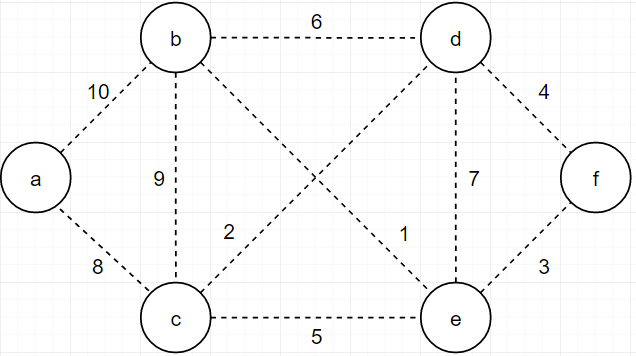
\includegraphics[height = 5 cm]{../entities/kruskal0}
\end{center}
Herefter betragtes kanten med vægt 1. Da den ikke resulterer i nogen cykler, tilføjes til den aktuelle minimum udspændede skov:
\begin{center}
    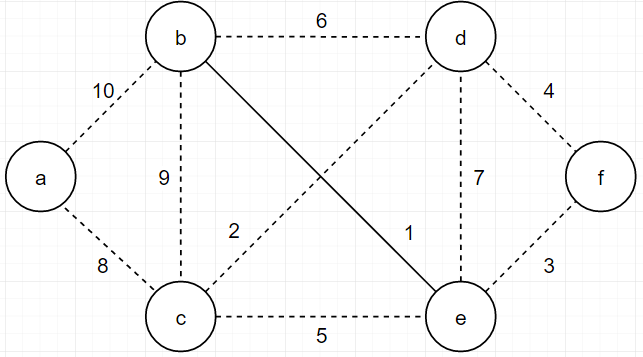
\includegraphics[height = 5 cm]{../entities/kruskal1}
\end{center}
Herefter betragtes kanten med vægt 2. Da den heller ikke resulterer i nogen cykler, tilføjes også den til den aktuelle minimum udspændede skov:
\begin{center}
    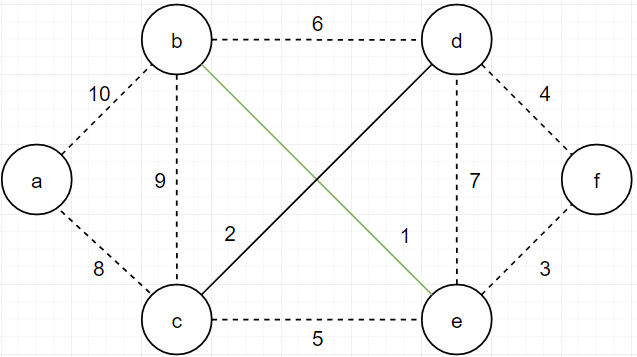
\includegraphics[height = 5 cm]{../entities/kruskal2}
\end{center}
Herefter betragtes kanten med vægt 3. Da heller ikke denne kant resulterer i nogen cykler, tilføjes også denne til den aktuelle minimum udspændede skov:
\begin{center}
    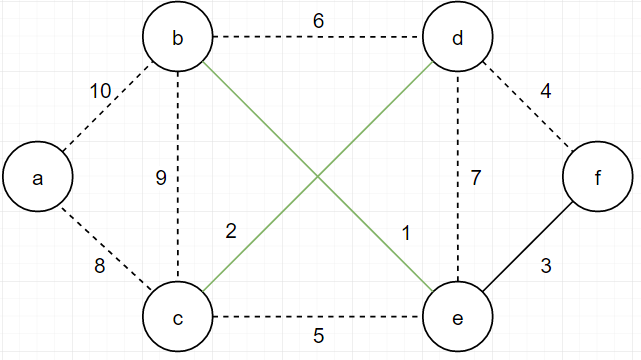
\includegraphics[height = 5 cm]{../entities/kruskal3}
\end{center}
Herefter betragtes kanten med vægten 4, som også tilføjes til den aktuelle minimum udspændede skov:
\begin{center}
    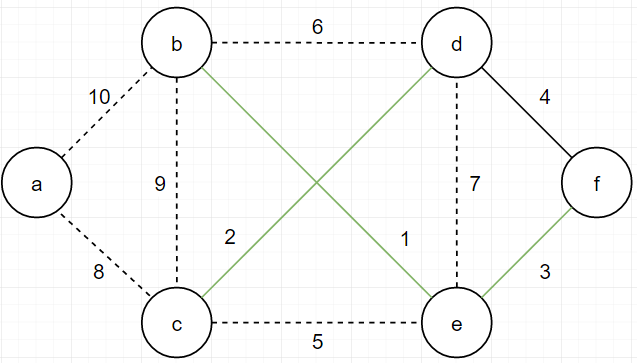
\includegraphics[height = 5 cm]{../entities/kruskal4}
\end{center}
Hertil betragtes kanten med vægten 5. Da denne kant resulterer i cyklen $(c, e), (e, f), (f, d), (d, c)$, bliver den ikke tilføjet til den aktuelle minimum udspændede skov:
\begin{center}
    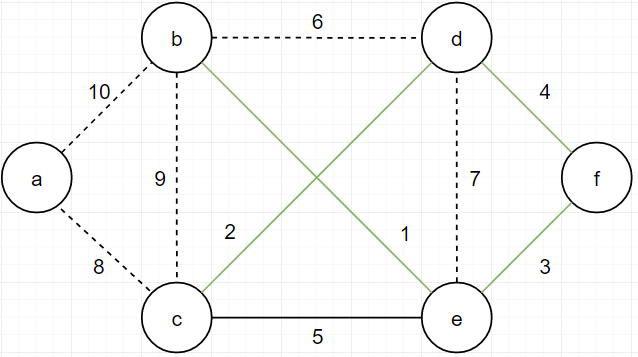
\includegraphics[height = 5 cm]{../entities/kruskal5}
\end{center}
Herefter kigges der på kanten med væten 6. Denne kan vil resultere i cyklen $(b, d), (d, f), (f, e), (e, b)$ bliver heller ikke denne tilføjet til den aktuelle minimum udspændede skov:
\begin{center}
    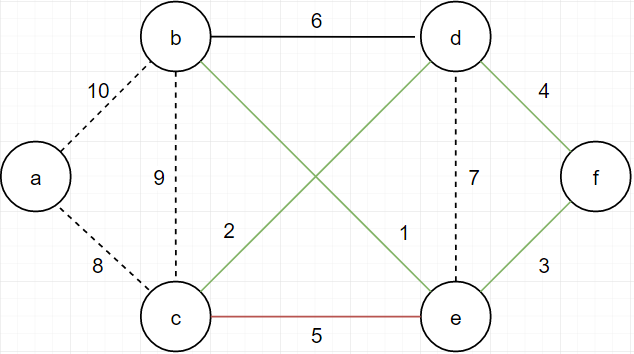
\includegraphics[height = 5 cm]{../entities/kruskal6}
\end{center}
Hertil betragtes kanten med vægt 7. Også denne kant vil resultere i en cykle, nemlig cyklen $(e, d), (d, f), (f, e)$. Derfor bliver den ikke tilføjet til den aktuelle minimum udspændede skov:
\begin{center}
    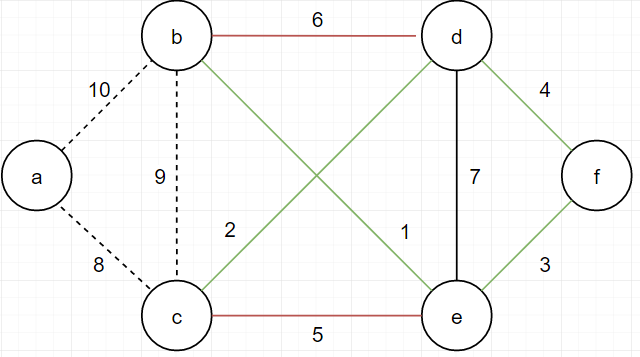
\includegraphics[height = 5 cm]{../entities/kruskal7}
\end{center}
Hertil bliver kanten med vægt 8 betragtet. Da denne kant ikke resulterer i nogen cykler, bliver den tilføjet til den aktuelle minimum udspændede skov:
\begin{center}
    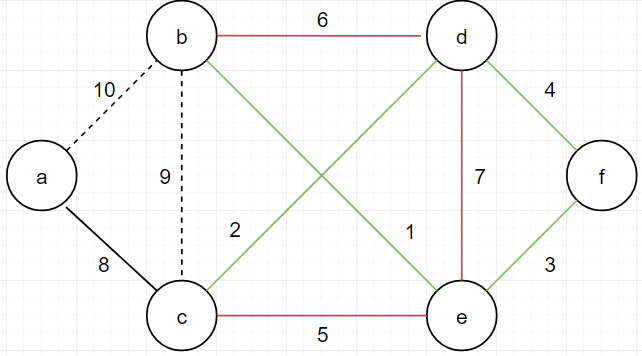
\includegraphics[height = 5 cm]{../entities/kruskal8}
\end{center}
Herefter bliver kanten med vægt 10 betragtet:
\begin{center}
    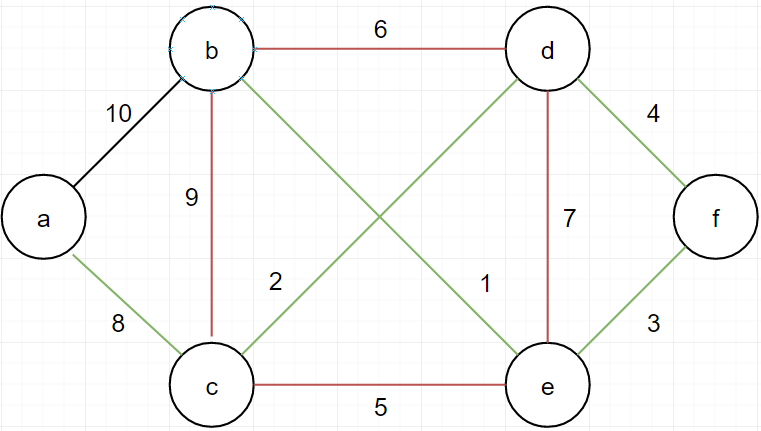
\includegraphics[height = 5 cm]{../entities/kruskal10}
\end{center}
Da denne kant vil resultere i en cyklus - nemlig $(a, b), (b, e), (e, f), (f, d), (d, c), (c, a)$, bliver den ikke tilføjet til den aktuelle minimum udspændede skov:
\begin{center}
    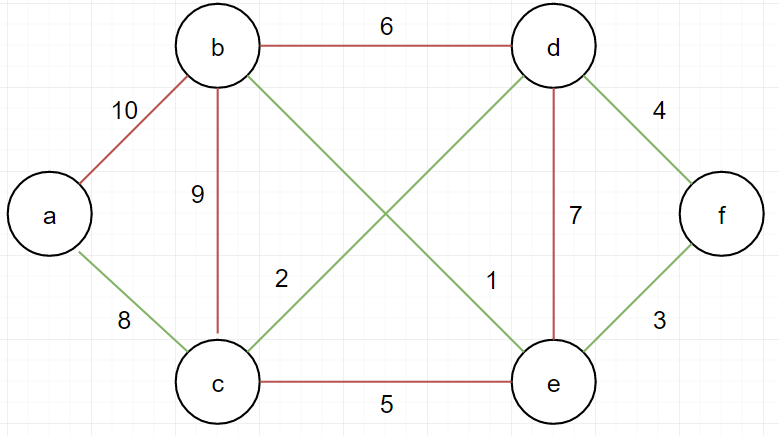
\includegraphics[height = 5 cm]{../entities/kruskal11}
\end{center}
Alt i alt ser det minimum udspændende træ ud som følgende:
\begin{center}
    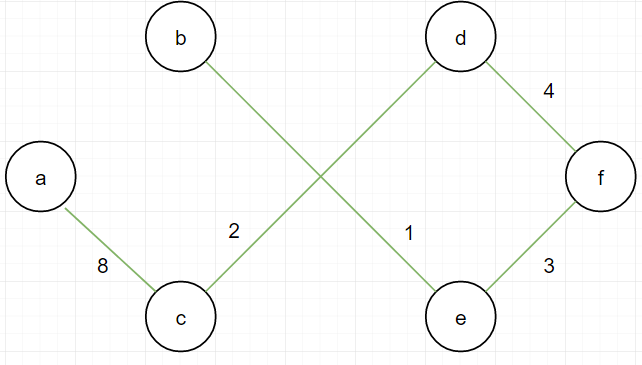
\includegraphics[height = 5 cm]{../entities/kruskal9}
\end{center}

\newpage

\subsection*{Del 4.2}
Det kan tydeligt vises ved et eksempel, at hvis væten af kanten $(d, f)$ ændres til 6, så vil $T$ ikke længere være et MST i $H$. Jeg vælger her at hoppe frem til den iteration, hvor kant $(d, f)$ ikke bliver taget med i den aktuelle minimum udspændede skov:
\begin{center}
    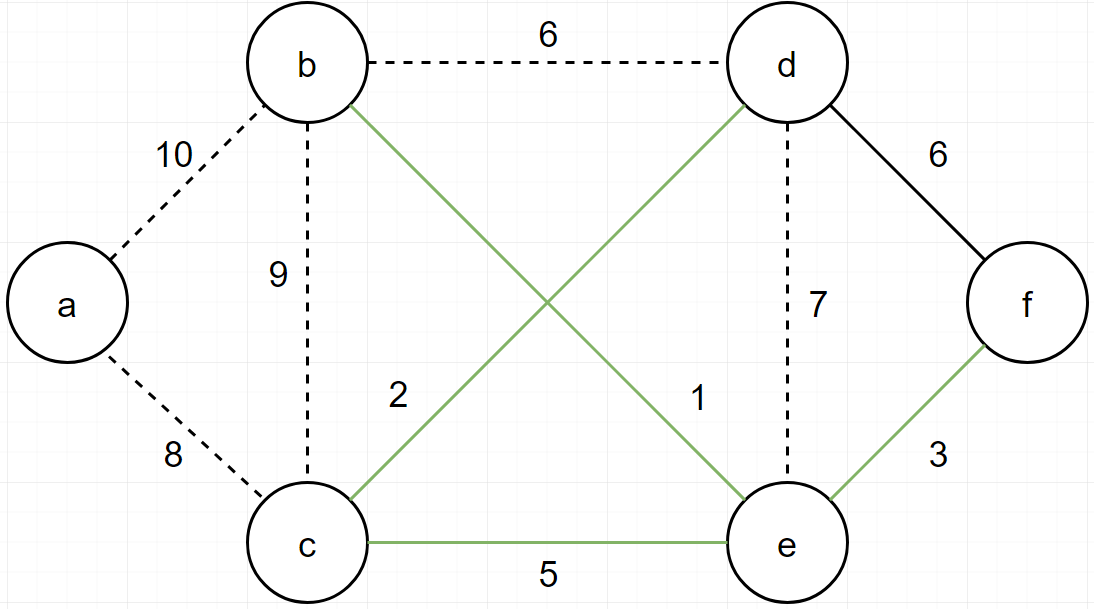
\includegraphics[height = 5 cm]{../entities/new_kruskal1}
\end{center}
Det er tydeligt at se her, at kanten $(d, f)$ ikke vil blive inkluderet i MST i $H$, idet vil så vil have cyklen $(c, d), (d, f), (f, e), (e, c)$. Derfor ender MST i $H$ ud med at være:
\begin{center}
    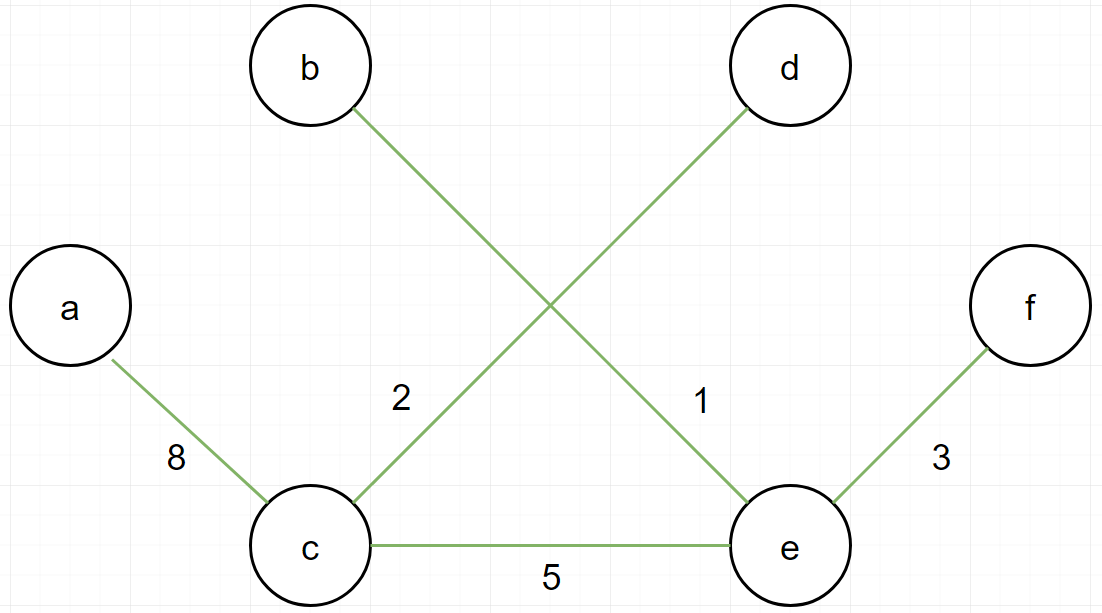
\includegraphics[height = 5 cm]{../entities/new_kruskal2}
\end{center}
hvilket ikke er lig $T$

\newpage

\subsection*{Del 4.3}
Ligesom ved delopgave 4.2 er det også tydeligt at vise ved hjælp af et eksempel, at hvis vægten af kant $(b, c)$ sættes til 3, så vil $T$ ikke længere være et MST i $H$. Nedenunder ses den iteration, hvor  $(b, c)$ bliver taget med i den aktuelle minimum udspændede skov, vilket den ellers ikke gør i $T$:
\begin{center}
    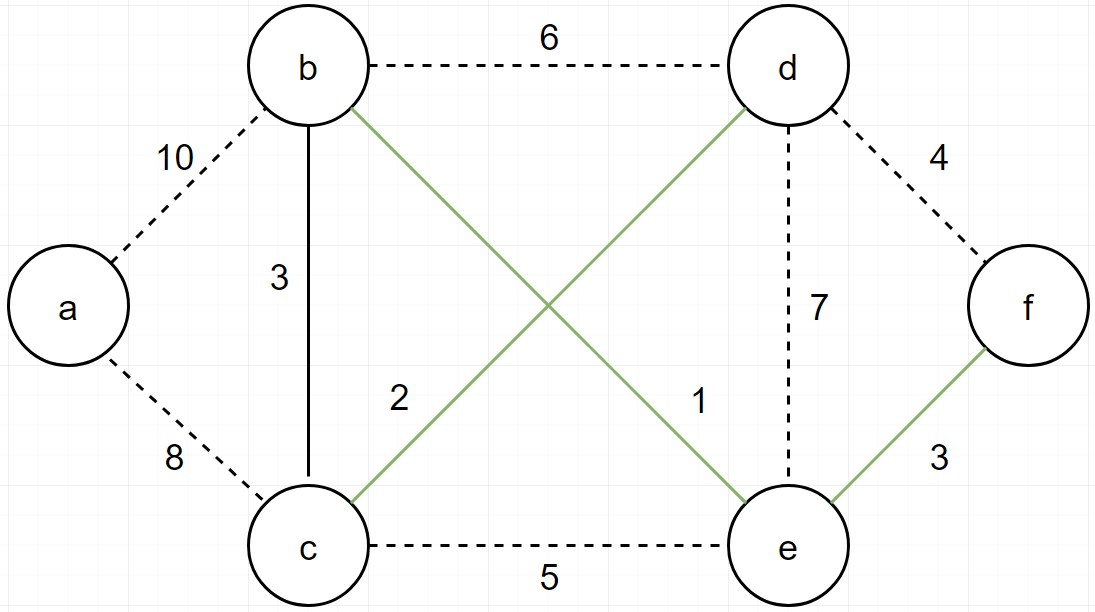
\includegraphics[height = 5 cm]{../entities/new_new_kruskal1}
\end{center}
Her er det tydeligt at se, at kanten $(b, c)$ faktisk bliver tilføjet til den aktuelle minimum udspændede skov, idet den er den kant med den mindste vægt der ikke er blevet betragtet endnu, samt den ikke skaber nogle cykler. Dette resulterer i, at algoritmen terminerer med følgende MST i $H$:
\begin{center}
    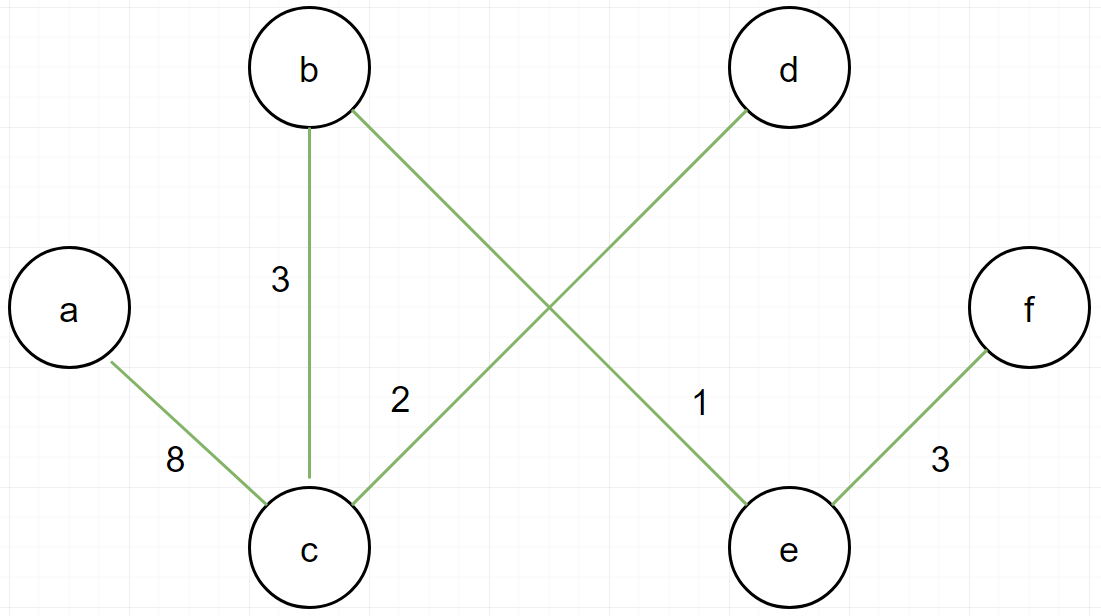
\includegraphics[height = 5 cm]{../entities/new_new_kruskal2}
\end{center}
hvilket ikke er lig $T$.

\newpage

\subsection*{Del 4.4}
Egenskaben lyder:
\begin{quote}
    Lad $T_1$ og $T_2$ betegne de to træer der opstår, hvis man fjerner $x$ fra $M$. Herved har vi, at for alle knuder, $u$ og $v$, der forbinder $T_1$ og $T_2$ skal vi have, at $k \leq w((u, v))$. 
\end{quote}
Da $x$ dog var med i $M$ må den altså være den kant der forbinder $T_1$ og $T_2$ med lavest vægt. Det vil altså sige, at egenskaben kan forkortest til uligheden 
$$k \leq w(x)$$ \\
Det første tilfælde kan bevises ved et modstrids bevis: \\
Vi antager, at der findes en sti i $G$ der forbinder $T_1$ og $T_2$ med en samlet vægt, der er lavere end $w(x)$. Men da vi ved, at $x$ er med i $M$ og $M$ er et MST, så er dette ikke muligt, og $w(x)$ må altså være den maksimale vægt en sti kan have der forbinder $T_1$ og $T_2$. Herved, hvis $M$ er et MST i $G'$, så må $k \leq w(x)$ gælde. \\
Det andet tilfælde kan der argumenteres for, idet det er muligt for den generiske MST-algoritme at finde $M$ i $G'$, idet den kan lave de samme \textit{cuts} der førte til $M$ i $G$ - pånær \textit{cut}'et der førte til at tilføje kant $x$ til $M$. Hertil mangler der altså kun en kant der forbinder de to træer $T_1$ og $T_2$. Laves der et cut over alle kanterne der forbinder de to træer, vil $x$ altså være det \textit{cut} med den laveste vægt, derved også være en \textit{light edge} og derved blive tilføjet til $M$. Ergo er det muligt for den generiske MST-algortime at finde $M$ i $G'$.

\newpage

\subsection*{Del 4.5}
Egenskaben kan beskrives ved uligheden:
$$k \geq w(x)$$
Der kan argumenteres for, at det første tilfælde gælder, idet vi ved at $x$ ikke er med $M$ idet den tilhørende vægt $w(x)$ er for "stor" til at blive inkluderet i $M$ - hertil gælder det altså, at for alle kanter, $y$, der forbinder de samme træer hvor $w(y) \geq w(x)$ gælder det altså også her, at vægten $w(y)$ er for står til at være med i $M$. \\
Ligesom i den forrige delopgave, kan der argumenteres fr, idet det er muligt for den generiske MST-aglrotime at finde $M$ i $G'$, idet den kan lave de samme \textit{cuts} der førte til $M$ i $G$ - pånær \textit{cut}'et der første til at tilføje kant $x$ til $M$. Hertil mangler der altså én kant til at forbinde de to træer $T_1$ og $T_2$. Laves der et cut over all kanterne der forbinder de to træer, vil $x$ aldrig være den kant med den laveste vægt, og vil derfor ikke blive tilføjet til $M$. Istedet vil den finde den kant der har den laveste vægt, hvilket også findes i $M$. Ergo, finder den altså frem til $M$.

\end{document}